% A good introduction to latex can be found here:
%    http://www.cse.ohio-state.edu/~hank/latex/lshort141.pdf

\documentclass[9.5pt]{extarticle}

\usepackage{full page}  % make the margins somewhat smaller than the default
\usepackage{graphicx}
\usepackage{amsmath}
\usepackage{indentfirst}
\usepackage{color}
\usepackage{cite}
\usepackage{wasysym}
\usepackage{amssymb}
\usepackage{multirow}
\usepackage{float}
\usepackage{lscape}
\usepackage{alltt} 
\usepackage{listings}
\usepackage{booktabs}
\usepackage{mathtools}
\usepackage{fancyhdr}
\usepackage[table,xcdraw]{xcolor}

\DeclarePairedDelimiter{\ceil}{\lceil}{\rceil}
\DeclarePairedDelimiter{\floor}{\lfloor}{\rfloor}

\definecolor{dkgreen}{rgb}{0,0.6,0}
\definecolor{gray}{rgb}{0.5,0.5,0.5}
\definecolor{mauve}{rgb}{0.58,0,0.82}


\usepackage{listings}  %  needed for source code listings

\lstset{frame=tb,
  language= java,
  aboveskip=1.5mm,
  belowskip=1.5mm,
  showstringspaces=false,
  columns=flexible,
  basicstyle={\small\ttfamily},
  keywordstyle=\color{blue},
  commentstyle=\color{dkgreen},
  stringstyle=\color{mauve},
  breaklines=true,
  tabsize=2,
  numbers=left,
  stepnumber=1,    
  firstnumber=1,
  numberfirstline=true
}
       

% set the document title, author, and date here.
%  once set, the \maketitle command (within the document)
%  will display them nicely
\title{Chess AI Assignment}
\author{Chua Zheng Fu Edrei}

\begin{document}
\maketitle

\section{Introduction}

In this report, I will implement a chess engine that uses minimax and alpha-beta pruning algorithm. I will describe the evaluation function. I will also make use of transposition table to improve the search efficiency of the chess engine. Experiments will be performed to verfiy the correctness of the algorithm and to compare its efficiency. Finally, I will present a literature review by Campell et al (2002) that describes the chess AI used in Deep Blue, the machine that defeated the World Chess Champion Garry Kasparov in a six-game match in 1997.


\section{Backbone}

I will first describe the backbone or the preparation work required before implementing the minimax or alpha-beta pruning algorithm.

\subsection{Check mate}

The code to check who won the game is straightforward: we simply check whose turn it is to play. The function to check who won the game is given in Listing 1.

\begin{lstlisting}[language=java,caption={Java function to check who won the game}]
private void checkGame(Position pos){
	if(pos.isMate()){
		if(pos.getToPlay() == 0){
			log("Game Over: Black wins!");
		}else{
			log("Game Over: White wins!");
		}
	}else if(pos.isStaleMate() || pos.isTerminal()){
		log("Game Over: Black and White draws");
	}
}
\end{lstlisting}

\subsection{Wrapper class}

The minimax and alpha-beta pruning algorithm are recursive and they are based on the score (``utility''). However, we will want to return the corresponding move eventually. Because Java only allow the return of a single output, I created a wrapper class \verb`node` that stores both the move and the utility. The wrapper class is given in Listing 2.\\

\begin{lstlisting}[language=java,caption={Wrapper class so that minimax and alpha-beta search can return multiple output}]
private class node{
	protected short move;
	protected int utility;

	public node(short move, int utility){
		this.move = move;
		this.utility = utility;
	}
}
\end{lstlisting}

\subsection{Iterative deepening}

The algorithm for minimax and alpha-beta pruning will also be implemented for increasing depth. This is worthwhile because for a chess game, the number of states increases exponentially with depth, and it is important to only search deeper if necessary. An iterative deepening search algorithm, similar to the one used in assignment 1, is applied for this purpose and the code is given in Listing 3.

\begin{lstlisting}[language=java,caption={Java code for Iterative deepening search}]
public short getMove(Position position) {
	aiPlayer = position.getToPlay();
	node bestMove = new node();
	
	for(int i=0; i<MAX_DEPTH; i++){
		try {
			CURR_DEPTH = i;
			bestMove = minimaxDecide(position);

			// short circuit for best move found
			if(bestMove.utility == WIN_UTILITY){
				return bestMove.move;
			}
		}catch(Exception e){
			e.printStackTrace();
		}
	}
	return bestMove.move;
}
\end{lstlisting}

\subsection{Cut-off Test, Utility function and Evaluation function}

A cut-off test is implemented to cut off further search and is based on whether a terminal position has been established or if a particular depth has been explored. The code is straightforward and is given in Listing 4.

\begin{lstlisting}[language=java,caption={Java code for cutoffTest}]
private boolean cutoffTest(Position pos, int depth){
	return (depth >= CURR_DEPTH || pos.isTerminal());
}
\end{lstlisting}

In addition, I implemented a utility function to calculate the score of the terminal position. The score is \verb`LOSS_UTILITY = Integer.MIN_VALUE` if the AI loses, \verb`WIN_UTILITY = Integer.MAX_VALUE` if the AI wins and \verb`DRAW_UTILITY = 0` for stale mate. The code is given in Listing 5. If neither case is true, an evaulation function based on the \verb`getMaterial` is called and it will assign a score based on the material value of the pieces that might be captured. The code is given in Listing 6.

\begin{lstlisting}[language=java,caption={Java code for utilityFun}]
private int utilityFun(Position pos){
	if(pos.isTerminal()){
		if(pos.isMate()) {
			if (pos.getToPlay() == aiPlayer){
				return LOSS_UTILITY; // aiPlayer has lost
			}else{
				return WIN_UTILITY; // aiPlayer won
			}
		}else{
			return DRAW_UTILITY; // either draw or stalemate
		}
	}else{
		return evalFun(pos);
	}
}
\end{lstlisting}

\section{Minimax}

A standard Minimax algorithm, similar to the one described in pp 166 of the book, is implemented. The algorithm consists of 3 parts. \verb`minimaxDecide`  returns the appropriate move after calling the recursive helper function \verb`minValue`. \verb`minValue` and \verb`maxValue` are recursive functions that call each other and assumes that the other player plays optimally. Optimal play for \verb`Max` is defined as maximising the worse-case outcome for \verb`Max`. The function for \verb`minimaxDecide` is given in Listing 6 and the function for \verb`minValue` is given in Listing 7. The function for \verb`maxValue` is not included in this report because it is very similar to that of \verb`minValue` and the details of the implementation can be found in MinimaxAI.java. The code for the transposition table is also included in Listing 7, but they will be further elaborated in section 5 of the report. Experiment and Testing will be described in section 6.

\begin{lstlisting}[language=java,caption={Java code for minimaxDecide for minimax algorithm}]
private node minimaxDecide(Position pos) throws Exception{
	short bestMove = Short.MIN_VALUE;
	int bestMoveUtility = LOSS_UTILITY;
	
	for(short move: pos.getAllMoves()){
		pos.doMove(move);
		int currMoveUtility = minValue(pos,1);
		if(currMoveUtility > bestMoveUtility){
			bestMoveUtility = currMoveUtility;
			bestMove = move;
		}
		pos.undoMove();
	}
	return new node(bestMove,bestMoveUtility);
}
\end{lstlisting}

\begin{lstlisting}[language=java,caption={Java code for minValue for minimax algorithm}]
private int minValue(Position pos, int depth) throws Exception{
	int min = WIN_UTILITY;
	incrementNodeCount();
	updateDepth(depth);

	if(transpose && transposition.containsKey(pos.getHashCode()) && transposition.get(pos.getHashCode()).depth > CURR_DEPTH){
		return transposition.get(pos.getHashCode()).score;
	}else if(cutoffTest(pos,depth)){
		int score = utilityFun(pos);
		if(transpose && (!transposition.containsKey(pos.getHashCode()) || transposition.get(pos.getHashCode()).depth < depth)) {
			transposition.put(pos.getHashCode(), new tableNode(score, depth));
		}
		return score;
	}

	for(short move: pos.getAllMoves()){
		pos.doMove(move);
		min = Math.min(min,maxValue(pos,depth+1));
		pos.undoMove();
	}
	return min;
}
\end{lstlisting}

\section{Alpha-Beta Pruning}

Alpha-beta pruning recognizes that when we have a lower bound for the value of the best choice found along the path of Min ($\beta$)  and when we have an upper bound for the value of the best choice found along the path of Max ($\alpha$), we do not need to consider subtree whose parent is known to be worse than the current $\alpha$ or $\beta$, and this pruning can save a lot of unnecessary search time. The algorithm consists of 3 parts and is similar to the pseudocode outlined in pp 170 of the book. \verb`alphaBetaSearch` returns the appropriate move after calling the recursive helper function \verb`minValue`. \verb`minValue` and \verb`maxValue` are recursive functions that call each other and assumes optimal play of the opponent. They are similar to the algorithm described in section 3, except that a lower bound and upper bound is included for pruning purposes. The function for \verb`minValue` is given in Listing 8. The function for \verb`alphaBetaSearch` is not included in this report because it is very similar to the one presented in Listing 6 abd \verb`maxValue` is not included because it is very similar to that of \verb`minValue`. The details for both functions can be found in AlphaBetaAI.java.  The code for the transposition table is also included in Listing 8, but will be further elaborated in section 5 of the report. Experiment and Testing will be described in section 6.

\begin{lstlisting}[language=java,caption={Java code for minValue for alpha beta pruning algorithm}]
private int minValue(Position pos, int depth, int alpha, int beta) throws Exception {

        int min = WIN_UTILITY;
        incrementNodeCount();
        updateDepth(depth);

        if(transpose && transposition.containsKey(pos.getHashCode()) && transposition.get(pos.getHashCode()).depth > CURR_DEPTH){
            int score = transposition.get(pos.getHashCode()).score;
            if(transposition.get(pos.getHashCode()).type == 0){
                return score;
            }else if(transposition.get(pos.getHashCode()).type < 0 && score >= beta){
                return score;
            }else if(transposition.get(pos.getHashCode()).type > 0 && score <= alpha){
                return score;
            }else if(beta <= alpha){
                return score;
            }
        }
        if(cutoffTest(pos,depth)){
            int score = utilityFun(pos);
            if(transpose && score <= alpha){
                transposition.put(pos.getHashCode(),new tableNode(score,depth,1));
            }else if(transpose && score >= beta){
                transposition.put(pos.getHashCode(),new tableNode(score,depth,-1));
            }else if(transpose){
                transposition.put(pos.getHashCode(),new tableNode(score,depth,0));
            }
            return score;
        }

        for(short move: pos.getAllMoves()){
            pos.doMove(move);
            min = Math.min(min,maxValue(pos,depth+1,alpha,beta));
            pos.undoMove();

            //pruning
            if(min <= alpha){
                return min;
            }
            beta = Math.min(beta,min);

        }
        return min;
    }
\end{lstlisting}

\section{Transposition Table}

A transposition table is implemented and it uses a hash map \verb`Map<Long,tableNode> transposition`. The details of the implementation are described by the TA Yu-Han in a piazza post. A wrapper class \verb`tableNode` is created so that three different pieces of information can be stored: 1. score (the score of the position); 2. depth (the depth of the search for getting the score) 3. type (-1 if the score is a lower bound, 0 if it is exact and 1 if it is an upper bound). For minimax search, all the scores will be exact and the type is unnecessary. \\

The basic idea of a transposition table is to store the score of the positions that have already been determined so that we can avoid doing duplicate work. Before we compute the score of a position, we query the position in the transposition table and check that the depth of the previous search is deeper than the current search. If the score is exact, we return the score directly. If the score is a lower bound and is at least $\beta$, we return the score too. Finally, if the score is an upper bound and is at most $\alpha$, we also return the score. By symmetry, we will store the score of a position after computing it into the transposition table. \\

The replacement scheme is straightforward: we replace the old information only when the old score is obtained by a smaller depth. This is because we want the information stored in the hash table to be the most optimal score that is obtained based on the deepest search possible. The implementation of the transposition table update and query is already included in the code given in Listing 7 and 8.

\section{Experiment and Results}

In this section, we will describe the experiment and results of the chess engine. I used the test cases 1 to 10 described by Yu-Han in a piazza post to established the accuracy of the chess engine, and I obtained the expected outcome. The test cases are given in Listing 9:

\begin{lstlisting}[language=java,caption={Test cases used in experiments and experimental outcome agrees with expected outcome}]
r5k1/p3Qpbp/2p3p1/1p6/q3bN2/6PP/PP3P2/K2RR3 b - - 0 1, black wins in 3
6k1/Q4pp1/2pq2rp/3p2n1/4r3/2PN4/P4PPP/2R2R1K b - - 0 1, black wins in 3
8/4B2p/7n/4pqpk/P2n1b2/R3P2P/2r3P1/1Q3R1K b - - 0 1, black wins in 3
2kr3r/1bbp1p2/p3pp2/1p4q1/4P3/PNN1PBP1/1PP3KP/1R1Q1R2 b - - 0 1, black wins in 3
5rk1/p4ppp/2b2q1P/7B/4p1Q1/5PR1/PPPb2R1/1K6 b - - 0 1, black wins in 3
3q2k1/1pp2pp1/7p/5b2/1P6/2Q2P2/r5PP/2BrRK1R b - - 2 25, black wins in 3
r2qk2r/pp6/2pbp3/2Pp1p2/3PBPp1/4PRp1/PP1BQ1P1/4R1K1 b kq - 0 20, black wins in 4
5r2/p1p1p1k1/1p2prpp/4R3/3P2P1/P1P1Q3/2q1R2P/6K1 b - - 1 28, black wins in 5
2rr2k1/Qp4pp/4bp2/4n3/4B3/1P2B1P1/P3q2P/RK5R b - - 1 24, black wins in 5
8/8/8/8/8/k1B5/BN6/K7 w - - 0 1, white wins in 6
\end{lstlisting}

Images of a game based on Test case 1 is given in Figure 1. Note the signs of intelligent play: BLACK is willing to sacrifice important chess pieces in order to force a check mate. This indicates that the untility function, as well as the minimax and alpha beta pruning algorithms, are working properly. BLACK in this case is the AlphaBetaAI while WHITE is RandomAI and \verb`MAX_DEPTH = 7`. The game is won in 3 moves.

\begin{figure}[H]
\centering
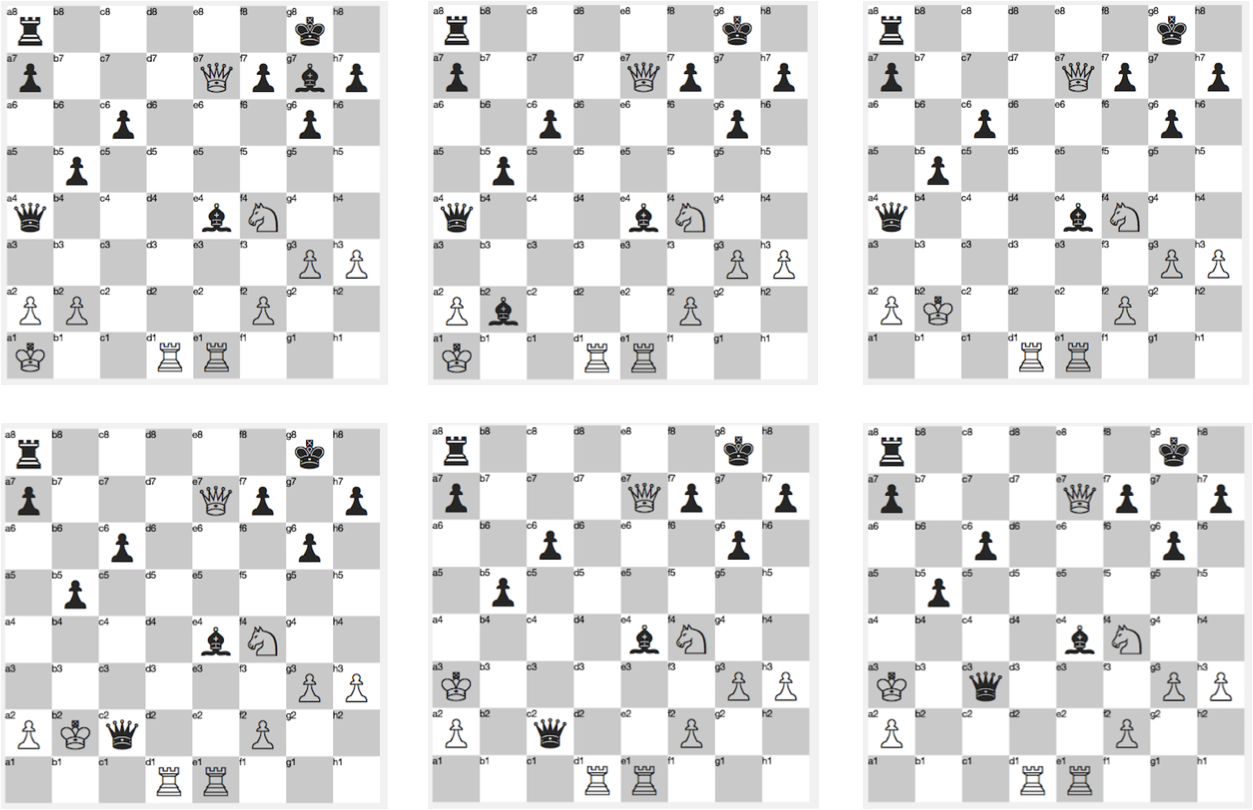
\includegraphics[scale=0.7]{game1.png}
\caption{Black wins in 3 moves. Starting position: r5k1/p3Qpbp/2p3p1/1p6/q3bN2/6PP/PP3P2/K2RR3 b - - 0 1 }
\label{Figure 1}
\end{figure}

The test case for the evaluation function is slightly more tricky since we have to ensure that the search doesn't end in a definitive state (win, lose or draw). To accomplish this, I used test case 9 and I change \verb`MAX_DEPTH = 3`. The game is shown below and we observed that the first few moves were made based on the evaluation function (material value of the pieces captured) since a definitive state is not available for a search depth of 3. Refer to Figure 2 for a visual representation of the game and Listing 10 for the corresponding Utility function value. We will label the sub images in Figure 2 from left to right, and top to bottom as 2a,2b,2c,2d,2e,2f,2g,2h,2i.\\



\begin{figure}[H]
\centering
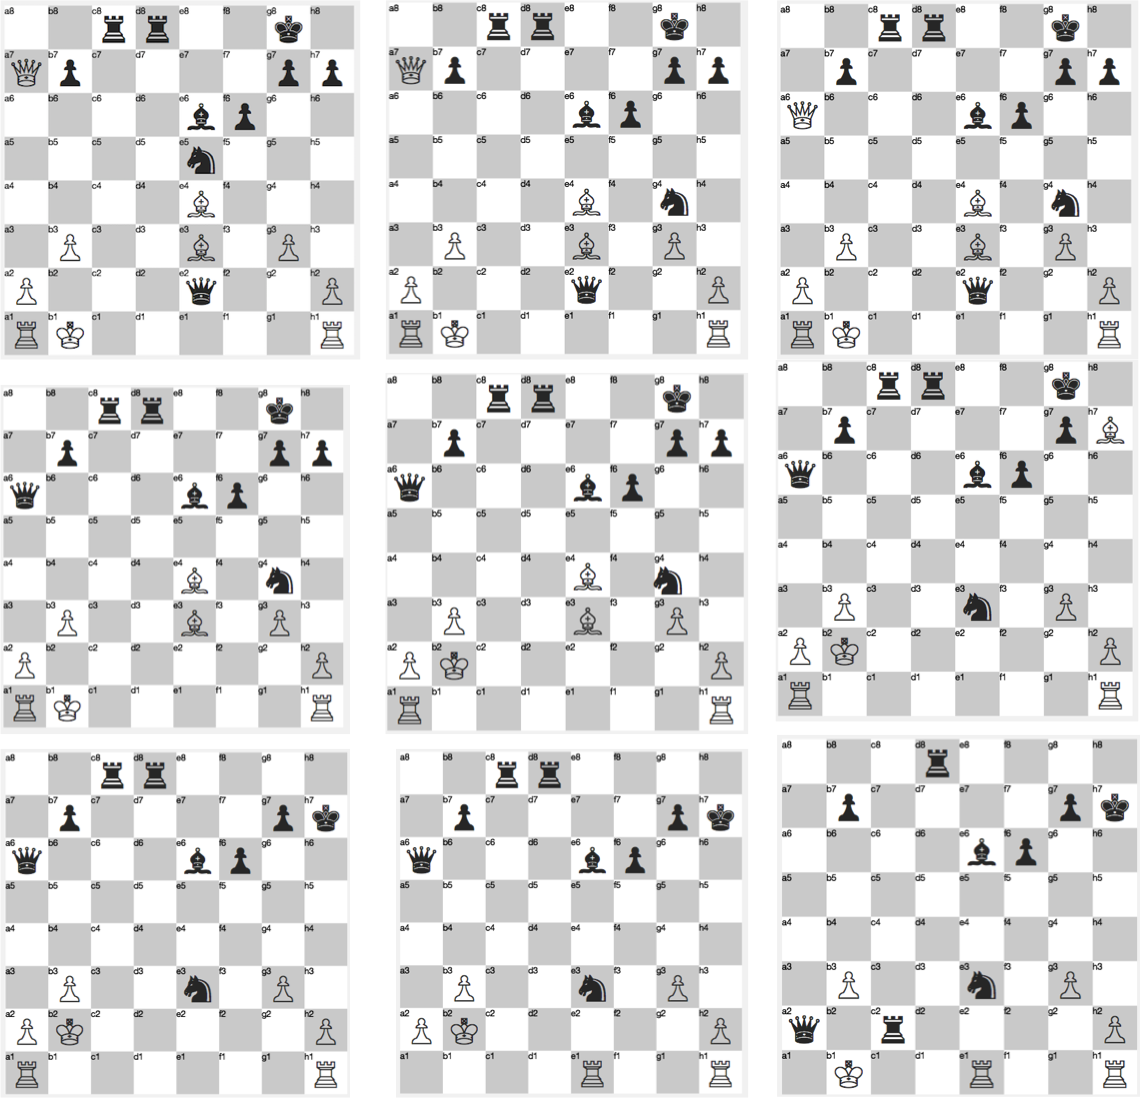
\includegraphics[scale=0.7]{game2.png}
\caption{Starting position: 2rr2k1/Qp4pp/4bp2/4n3/4B3/1P2B1P1/P3q2P/RK5R b - - 1 24}
\label{Figure 2}
\end{figure}

\begin{lstlisting}[language=java,caption={Utility function for game in Figure 2}]
Utility function yield score: -125
Utility function yield score: 775
Utility function yield score: 1100
Utility function yield score: 1425
Utility function yield score: 1425
Utilty function yield score: 2147483647
\end{lstlisting}

Observe that at the beginning, BLACK does not have any meaningful move to make and thus it just move in a way to maximize the utility score. At 2c, BLACK has two options: capture the rock at e3 with the knight at g4 or capture the queen at a6 with the queen at e2. It chooses the latter, which demonstrated intelligence because it prevents its queen from being captured in the next round and also the material value of a queen is higher than a rock (this would yield a higher utility function). Again, at 2e, the knight at g4 chooses to capture the rock at e3 because it has the highest material value compared to the other pieces that can be captured. Finally, we note that at the last step, BLACK is not interested in the material value of any potential pieces that can be captured since it realises that it can force a checkmate (note the utility score is \verb`Integer.MAX_VALUE`.\\

Finally, I also attempt to compare the performance of the two algorithms, with and without the implementation of transposition table. The test is conducted using Test case 1 to 5. I note that alpha-beta pruning with transposition table explore the least number of nodes, followed by alpha-beta without transposition, then minimax with transposition and finally minimax without transposition. The improvement by using a transposition table seems to be only incremental because as Yu-Han noted that if the evaluation is very efficient (which it is since I have decided to use the \verb`getMaterial` inbuild function), the transposition table will only be useful near the top of the search tree. For Test case 1 (Figure 1), I note that alpha beta pruning explores for the second move 16855 nodes for a search depth of 3 while minimax explores 43886 nodes for a similar move and search depth for the same position. This represents an approximately 62\% improvement in runtime performance. On the other hand, transposition table only improves the number of nodes to 37144 for the same move and search depth for the minimax algorithm, representing only a 15\% improvement. Transposition table for alpha beta pruning has similar performance as that for minimax.\\

Therefore, the conclusion is that while transposition table improves the runtime performance by some amount, the most significant improvement comes from using alpha beta pruning. Alpha beta pruning, combined with transposition table, yield the best performance overall.\\

\section{Literature Review}

I choose the article Deep Blue by Campell et al. 2002 (M. Campell, A. Joseph, F. Hsu (2002) ``Deep Blue'', Artificial Intelligence 134: 57 - 83) because I have always been interested in how IBM created the first chess engine that defeated the World Chess Champion Garry Kasparov in a six-game match in 1997.\\

Campell et al highlighted a few areas that resulted in the improvement in performance of Deep Blue that resulted in the win in 1997 (there is another version of Deep Blue that was defeated by Kasparov in 1996). Some of the reasons included: a single-chip chess search engine, a massively parallel system with multiple levels of parallelism, a strong emphasis on search extensions, a complex evaluation function, and effective use of a Grandmaster game database. I will emphasis on the last two in this section.\\

Firstly, I find it interesting that the chess engine for Deep Blue is very similar to the one we built for this assignment: essentially, both uses a search algorithm. Deep Blue uses a negascout algorithm, with transposition table and move ordering. Another strength is its ability to perform parallel computing, which improves the run time tremendously. This indicates that the hardware for building a AI is just as important as the software.\\

Two significant improvements involved the use of a complex evaluation function and a good opening book. The evaulation function uses a hill-climbing approach. In addition, it also has the ability to make good approximation instead of evaluating the exact score (and a good heuristic to decide which approach will be better), thus optimizing the run time. Finally, Deep Blue uses an opening book reated by hand, primarily by Grandmaster Joel Benjamin, with assistance from Grandmasters Nick De Firmian, John Fedorowicz, and Miguel Illescas. The book consisted of about 4000 positions. One significant weakness of the AI is that it won't play well at the beginning of the game. The material value of the board only changes with a capture, and captures are rare at the beginning. An opening book is able to circumvent this weakness.\\

\end{document}